\section{Preliminaries}
\label{sec:preli}
% motivation
In the OppNets,
the messages, e.g., advertisements, urgent notifications,
reports and tasks,
always need to be disseminated
to the specific group of users.
As an example, the source node $src$
should disseminate the message $m$,
which will exist from $0$ to $T$,
to the relay nodes,
e.g., vehicles or pedestrians.
There are $N$ relay nodes in the network,
which can replicate, store $m$ and send it further.
Thus the potential coverage area of the message
can be broadened by this network.
To encourage the collaboration of relay nodes,
$src$ should reward the relay node $n_{i}$
$(1 \le i \le N)$ based on the message carrying time,
which means the maximum time-interval
starts from the replication time $\tau_{i}^{s}$
to $T$.
%which starts from the replication time $\tau_{i}^{s}$
%to the message lifetime $T$.
%during which the message are carried by $n_{i}$.
%The message carrying time
%ranges from the replication time ($\tau_{i}$)
%to the message lifetime ($T$).
Since $\tau_{i}^{s}$ is recorded by $src$
at the contact between $src$ and $n_{i}$,
$src$ can calculate the reward
as $\beta (T-\tau_{i}^{s})$, where $\beta$ is the reward per second.
%$n_{i}$ contacts $src$ and replicates $m$.
%Since the message only can be replicated
%from $src$ to the relay node in this paper,
%$src$ can record the replication time $\tau_{i}$.

\begin{figure}
  \centering
  {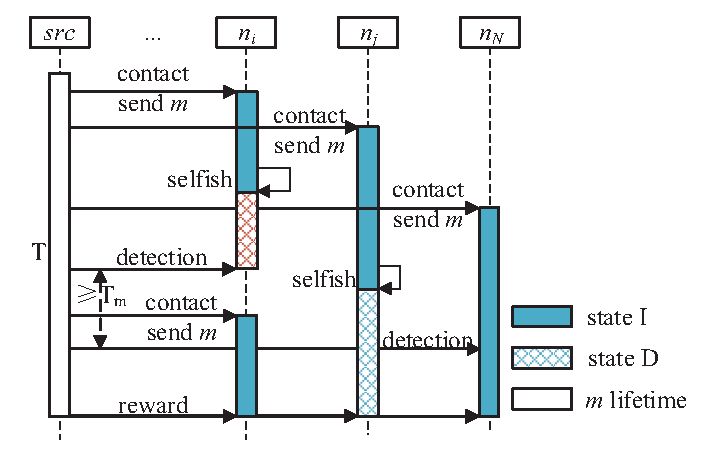
\includegraphics[width=0.47\textwidth]{fig/schedule.eps}}
     \caption{Sate transition of behaviors in time dimension.}
     \label{fig:schedule}
\end{figure}
However, $n_{i}$ may discard $m$
% immediately after the contact
to earn the reward without carrying $m$,
which is the main type of
the selfish behaviors considered in this paper.
To mitigate the behaviors,
$src$ adopts the detection,
%, which is the cost of selfish behaviors.
which can be conducted as follows:
$1$) $src$ selects a detected relay node $n_{r}$
from the $N$ node set randomly;
$2$) $src$ determines the random segment of the message $m_{+}$;
$3$) $src$ sends the query about the checksum of $m_{+}$
to $n_{r}$ via cellular networks 
(or other Internet access technologies);
$4$) If $src$ receives the correct checksum after $T_{m}$,
$n_{r}$ is not a selfish node;
otherwise, $n_{r}$ is a selfish node.
For example, if $n_{i}$ is identified
as a selfish node at time $\tau_{i}^{d}$,
the reward will be computed as $\beta(\tau_{i}^{d} - \tau_{i}^{s})$,
which means that $n_{i}$ will not receive the reward
from $\tau_{i}^{d}$.
The whole process,
including contacts, detections and rewards,
is shown in Fig.~\ref{fig:schedule}.
State $I$ means that the nodes carry $m$.
State $D$ denotes that the nodes have discarded $m$.
Other nodes stay in state $R$.
The contact can make the node,
which is in state $R$ or in state $D$,
transit into state $I$.
The selfish behavior encourages the node to discard the message,
which can still receive the reward from $src$
before being detected.
After the message lifetime,
the reward can be calculated according to
the contacts and the detections recorded in $src$.
In this paper, we propose the optimal random detection strategy
to reduce the detection cost 
caused by the frequent communications through cellular networks
and improve the reward utilization ratio.
%
%to achieve the tradeoff between
%the cost of the random detections and
%the wasted reward of the selfish behaviors.

%1.Poisson process of contacts
%2.Poisson process of being selfish
$E(R(t))$ denotes the expected number of the relay nodes,
which have not contacted $src$ before time $t$.
$E(I(t))$ denotes the expected number of infected relay nodes,
which still carry the message at time $t$.
$E(D(t))$ denotes the expected number of selfish relay nodes,
which have discarded the message 
but are still not found by time $t$.
Similar to \cite{DBLP:journals/tcss/WuDH18} and \cite{CC2007PerfAnaly},
the contacts between any two nodes
can be adequately modeled as Poisson process,
in which the contact rate is $\lambda$.
The total number of relay nodes is $N$,
and $N=R(t)+I(t)+D(t)$, $\forall t \in [0, T]$.
We also assume the rate of a node getting into selfish mode
from state $I$
is the constant parameter $\rho$.
The detection rate $U(t)$,
which means the detections speed at different time,
satisfies $0 \le U(t) \le U_{m}$, $\forall t \in [0, T]$.
For instance, if the minimal detection cycle
$T_{m}$ is that $2$s,
the maximal frequency of detection is
$U_{m} = \frac{1}{T_{m}} = 0.5$ per second.
To simplify the denotations,
we use $R(t)$, $I(t)$ and $D(t)$ to
replace $E(R(t))$, $E(I(t))$ and $E(D(t))$,
respectively.
%Then the main objective of our work is
%to solve the following problem,
The total reward paid to all relay nodes by $src$ is
\begin{equation}
\begin{small}
\label{eq:reward}
\begin{aligned}
P &= \int_{0}^{T} \beta \big( I(t) + D(t) \big)dt,
\end{aligned}
\end{small}
\end{equation}
where $\beta$ is the reward of unit time
paid to a node carrying the message.
$\int_{0}^{T} D(t) dt$ is proportional to the wasted reward.

The optimal random detection problem
in this paper can be formulated as:
\begin{equation}
\begin{small}
\label{eq:obj}
\begin{aligned}
Min: J &= \int_{0}^{T} \big( (1-\alpha) D(t) + \alpha U(t) \big) dt,
\end{aligned}
\end{small}
\end{equation}
which minimizes the linear combination of
the wasted reward and the detection cost through the weight $\alpha$,
$0 < \alpha < 1$.

